\chapter{Testing e valutazione sul campo dell'usabilità}
\raggedright{\section{Codice xUnit}}
Di seguito viene riportato il codice dartUnit per 4 metodi non banali che abbiano almeno due parametri.\\

\raggedright{\subsection{Unit Testing: Creazione Categoria}}
\lstinputlisting[language=Java]{dartUnit/creaCategoria.dart}

\newpage
\raggedright{\subsection{Unit Testing: Ricerca di un Riferimento}}
\lstinputlisting[language=Java]{dartUnit/ricercaRiferimento.dart}
\newpage
\raggedright{\subsection{Unit Testing: Calcolo hash}}
\lstinputlisting[language=Java]{dartUnit/calcoloHash.dart}
\raggedright{\subsection{Unit Testing: Regitrazione}}
\lstinputlisting[language=Java]{dartUnit/registrazione.dart}
\newpage
\raggedright{\subsection{Strategie adottate per la progettazione dei test}}
Tali unità di test sono state implementate mediante un approccio Black Box, anche se il codice sorgente era ovviamente disponibile. Questo perché abbiamo preferito testare il comportamento esterno dell'applicativo, senza doverci focalizzare sulle sfaccettature del codice. \\
Abbiamo deciso di presentare quattro unità di test tra i tanti metodi che sarebbero stati maggiormente utilizzati in Alexandria: un metodo per la creazione di una categoria, uno per la ricerca di un riferimento, uno per la creazione di un riferimento e infine uno per l'aggiunta di una citazione. In particolare, sono stati individuate tali classi d'equivalenza:

\begin{table}[H]
\begin{tabular}{|l|l|l|l|}
\hline
\textbf{creazioneCategoria}  &                           &                           &                          \\ \hline
String nome         & CE1: \{""\} n. v.         & CE2: \{"abc"\} val.       &                          \\ \hline
int user\_id        & CE3: \{minInt, -1\} n. v. & CE4: \{0, maxInt\} val.   &                          \\ \hline
int? superCategoria & CE5: \{null\} val.        & CE6: \{minInt, -1\} n. v. & CE7:  \{0, maxInt\} val. \\ \hline
\end{tabular}
\end{table}

\begin{table}[H]
\begin{tabular}{|l|l|l|l|}
\hline
\textbf{ricercaRiferimento}                      &                       &                              &                                \\ \hline
String? titolo                          & CE1: \{null\} val.    & CE2: \{""\} n. v.            & CE3: \{"abc"\} val.            \\ \hline
int? doi                                & CE4: \{null\} val.    & CE5: \{minInt, maxInt\} val. &                                \\ \hline
List\textless{}Categoria\textgreater c  & CE6: \{{[}{]}\} val.  & CE7: \{{[}1, .., n{]}\} val. &                                \\ \hline
List\textless{}tipo\_enum\textgreater t & CE8: \{{[}{]}\} n. v. & CE9: \{{[}1, .., 5{]}\} val. & CE10: \{{[}6, .., n{]}\} n. v. \\ \hline
\end{tabular}
\end{table}

\begin{table}[H]
\begin{tabular}{|l|l|l|}
\hline
\textbf{registrazioneUtente}     &                           &                         \\ \hline
String username         & CE1: \{""\} n. v.       & CE2: \{"abc"\} val.     \\ \hline
String unhashedPassword & CE3: \{""\} n. v. & CE4: \{"abc"\} val. \\ \hline
String nome             & CE5: \{""\} n. v.         & CE6: \{"abc"\} val.     \\ \hline
String cognome          & CE7: \{""\} n. v.         & CE8: \{"abc"\} val.     \\ \hline
String email            & CE9: \{""\} n. v.         & CE10: \{"abc"\} val.    \\ \hline
\end{tabular}
\end{table}
\begin{table}[H]
\begin{tabular}{|l|l|l|}
\hline
\textbf{calculateHash}  &                           &                         \\ \hline
String unhashedPassword & CE1: \{""\} n. v.       &  CE2: \{"abc"\} val.                       \\ \hline
String salt    & CE3: \{""\} n. v. & CE4: \{"abc"\} val. \\ \hline
\end{tabular}
\end{table}
Il criterio di copertura utilizzato è la \textit{\gls{Weak Equivalence Class Testing}}.
Le caratteristiche individuate per ogni classe d'equivalenza rispecchiano i casi limite dei possibili valori che un parametro della funzione possa assumere. 
\newpage
\raggedright{\section{Valutazione dell'usabilità sul campo}}
A prodotto finito, ci siamo avvalsi dell'uso di \href{https://analytics.google.com/analytics/web/}{Google Analytics} per analizzare in dettaglio le interazioni con gli utenti e il comportamento dell'applicazione una volta collegato con il server \gls{AWS}. In particolare, sono stati generati i seguenti file di log durante le fasi di valutazione dell'usabilità:

\begin{figure}[H]
    \centering
    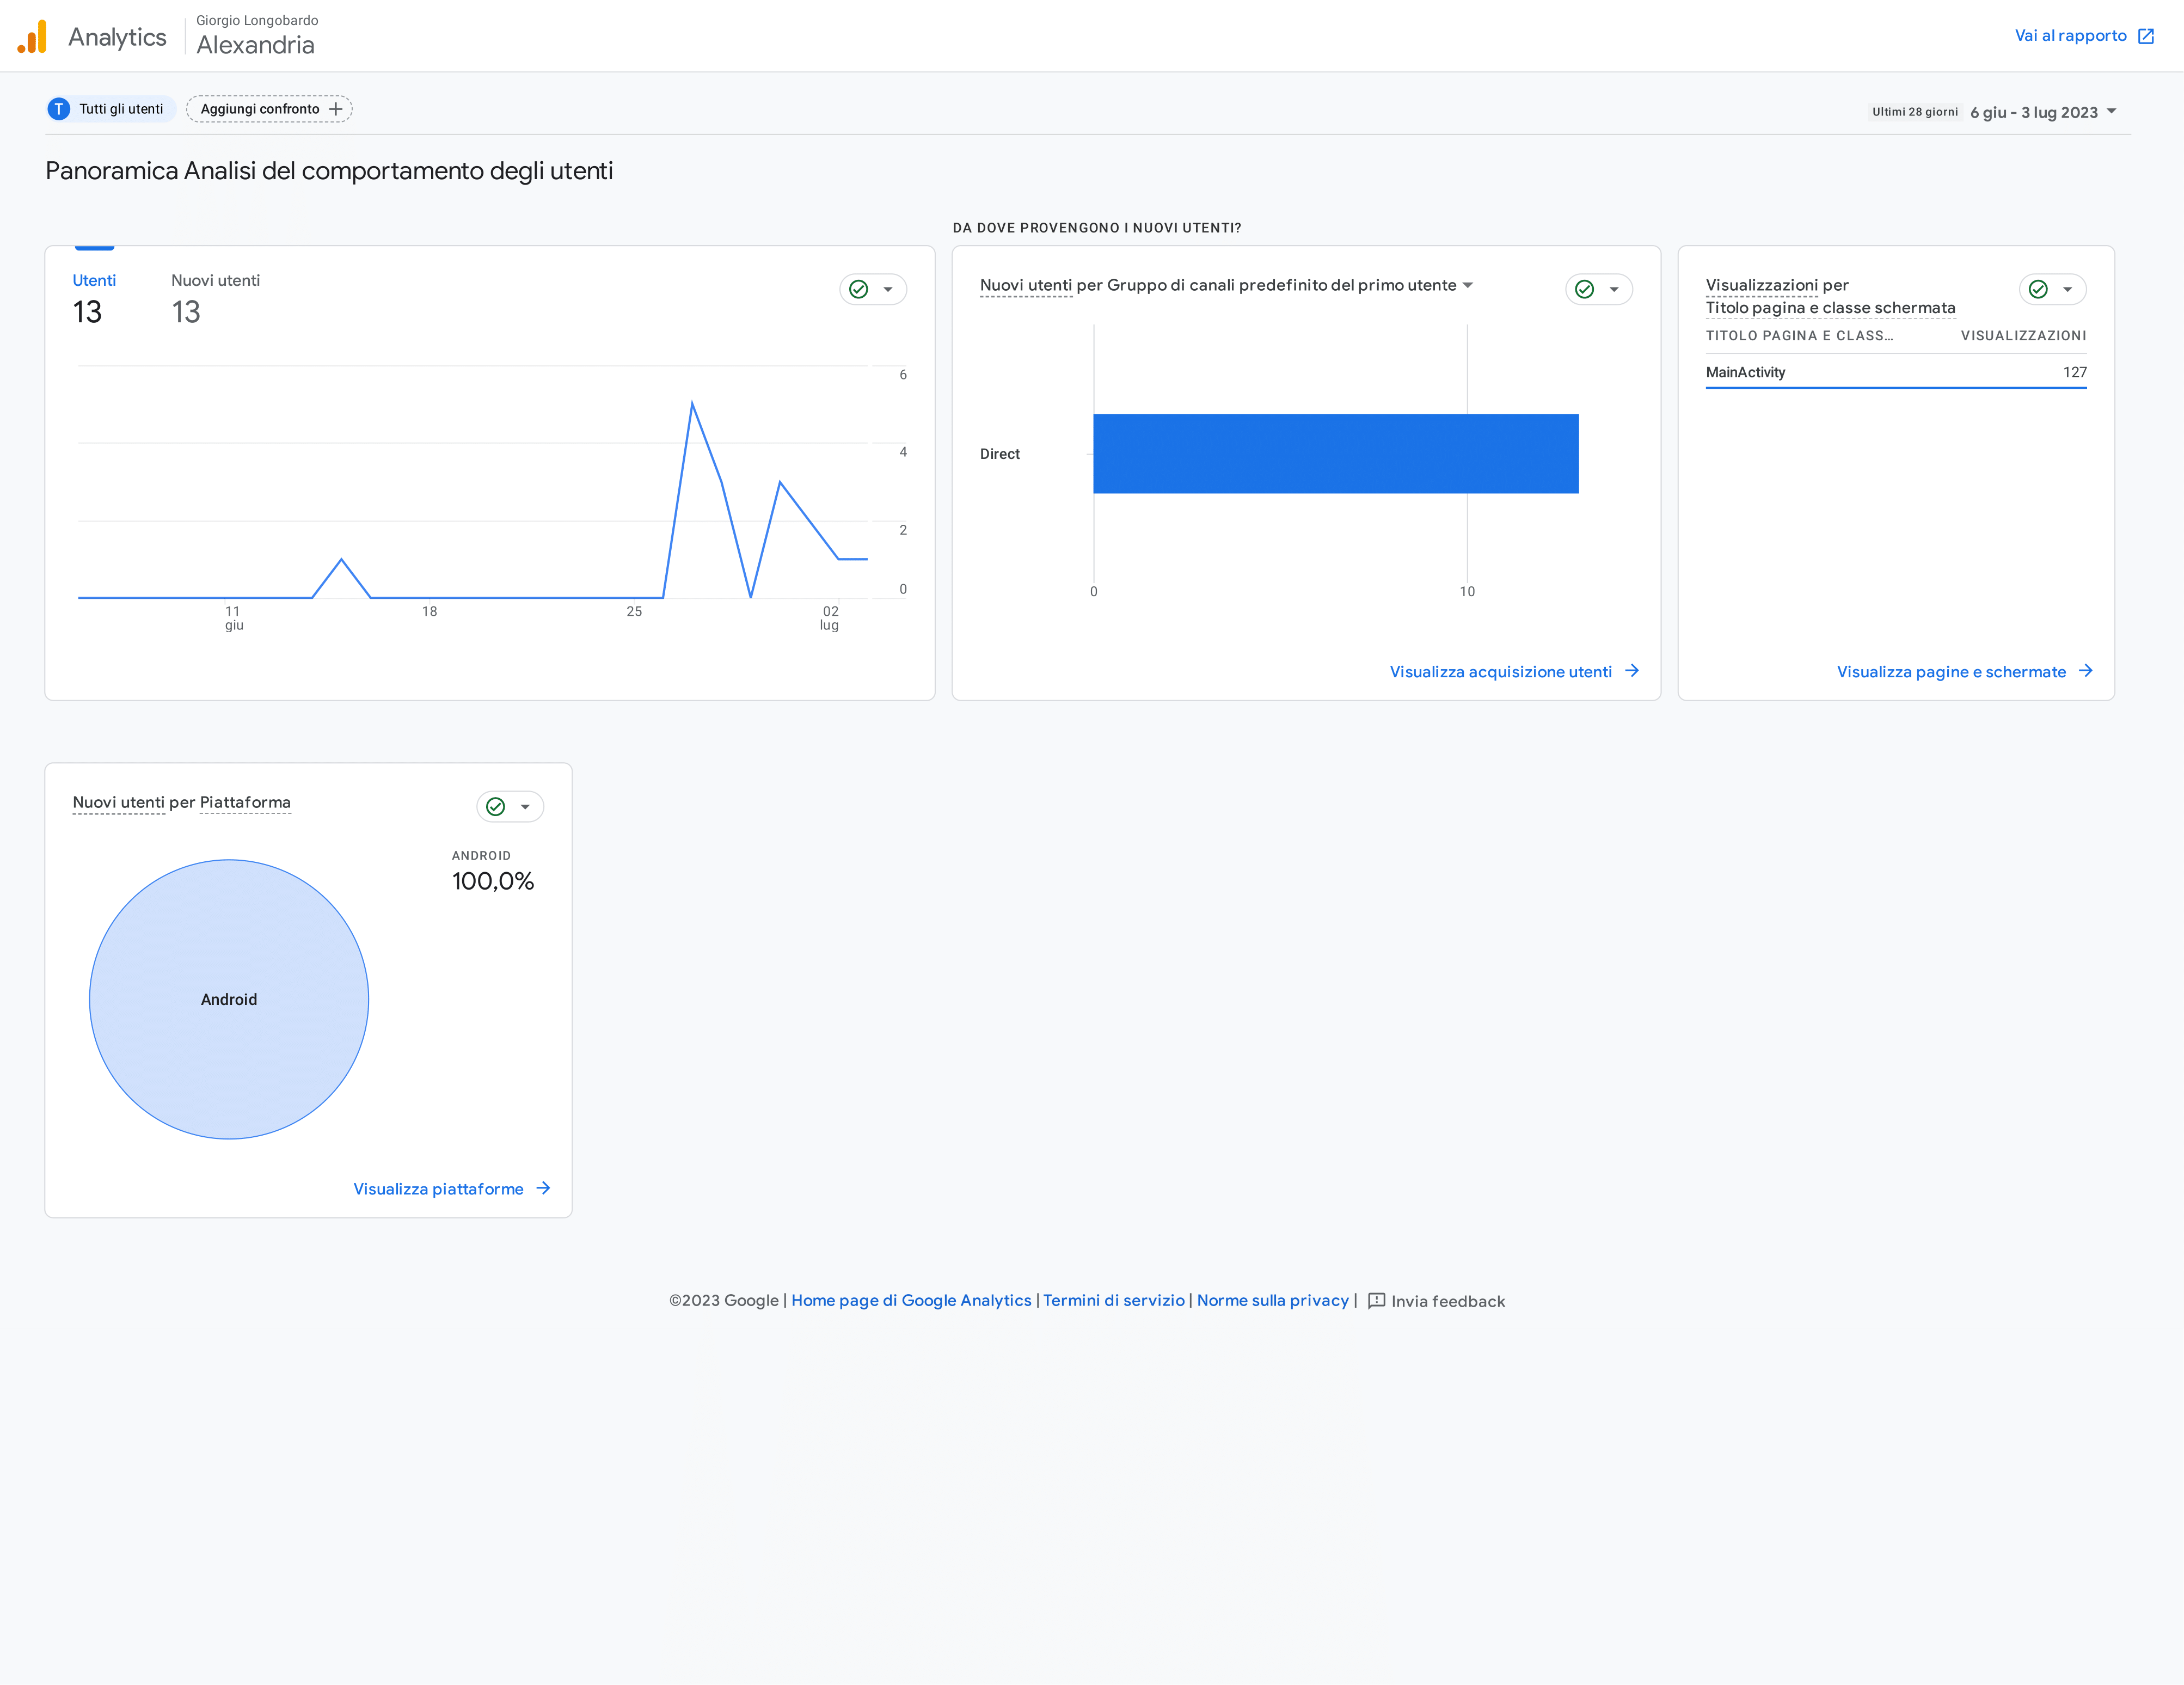
\includegraphics[width=0.99\textwidth]{Immagini/Alexandria/Report/panoramica-1.png}
    \caption{Panoramica generale}
\end{figure}

\begin{figure}[H]
    \centering
    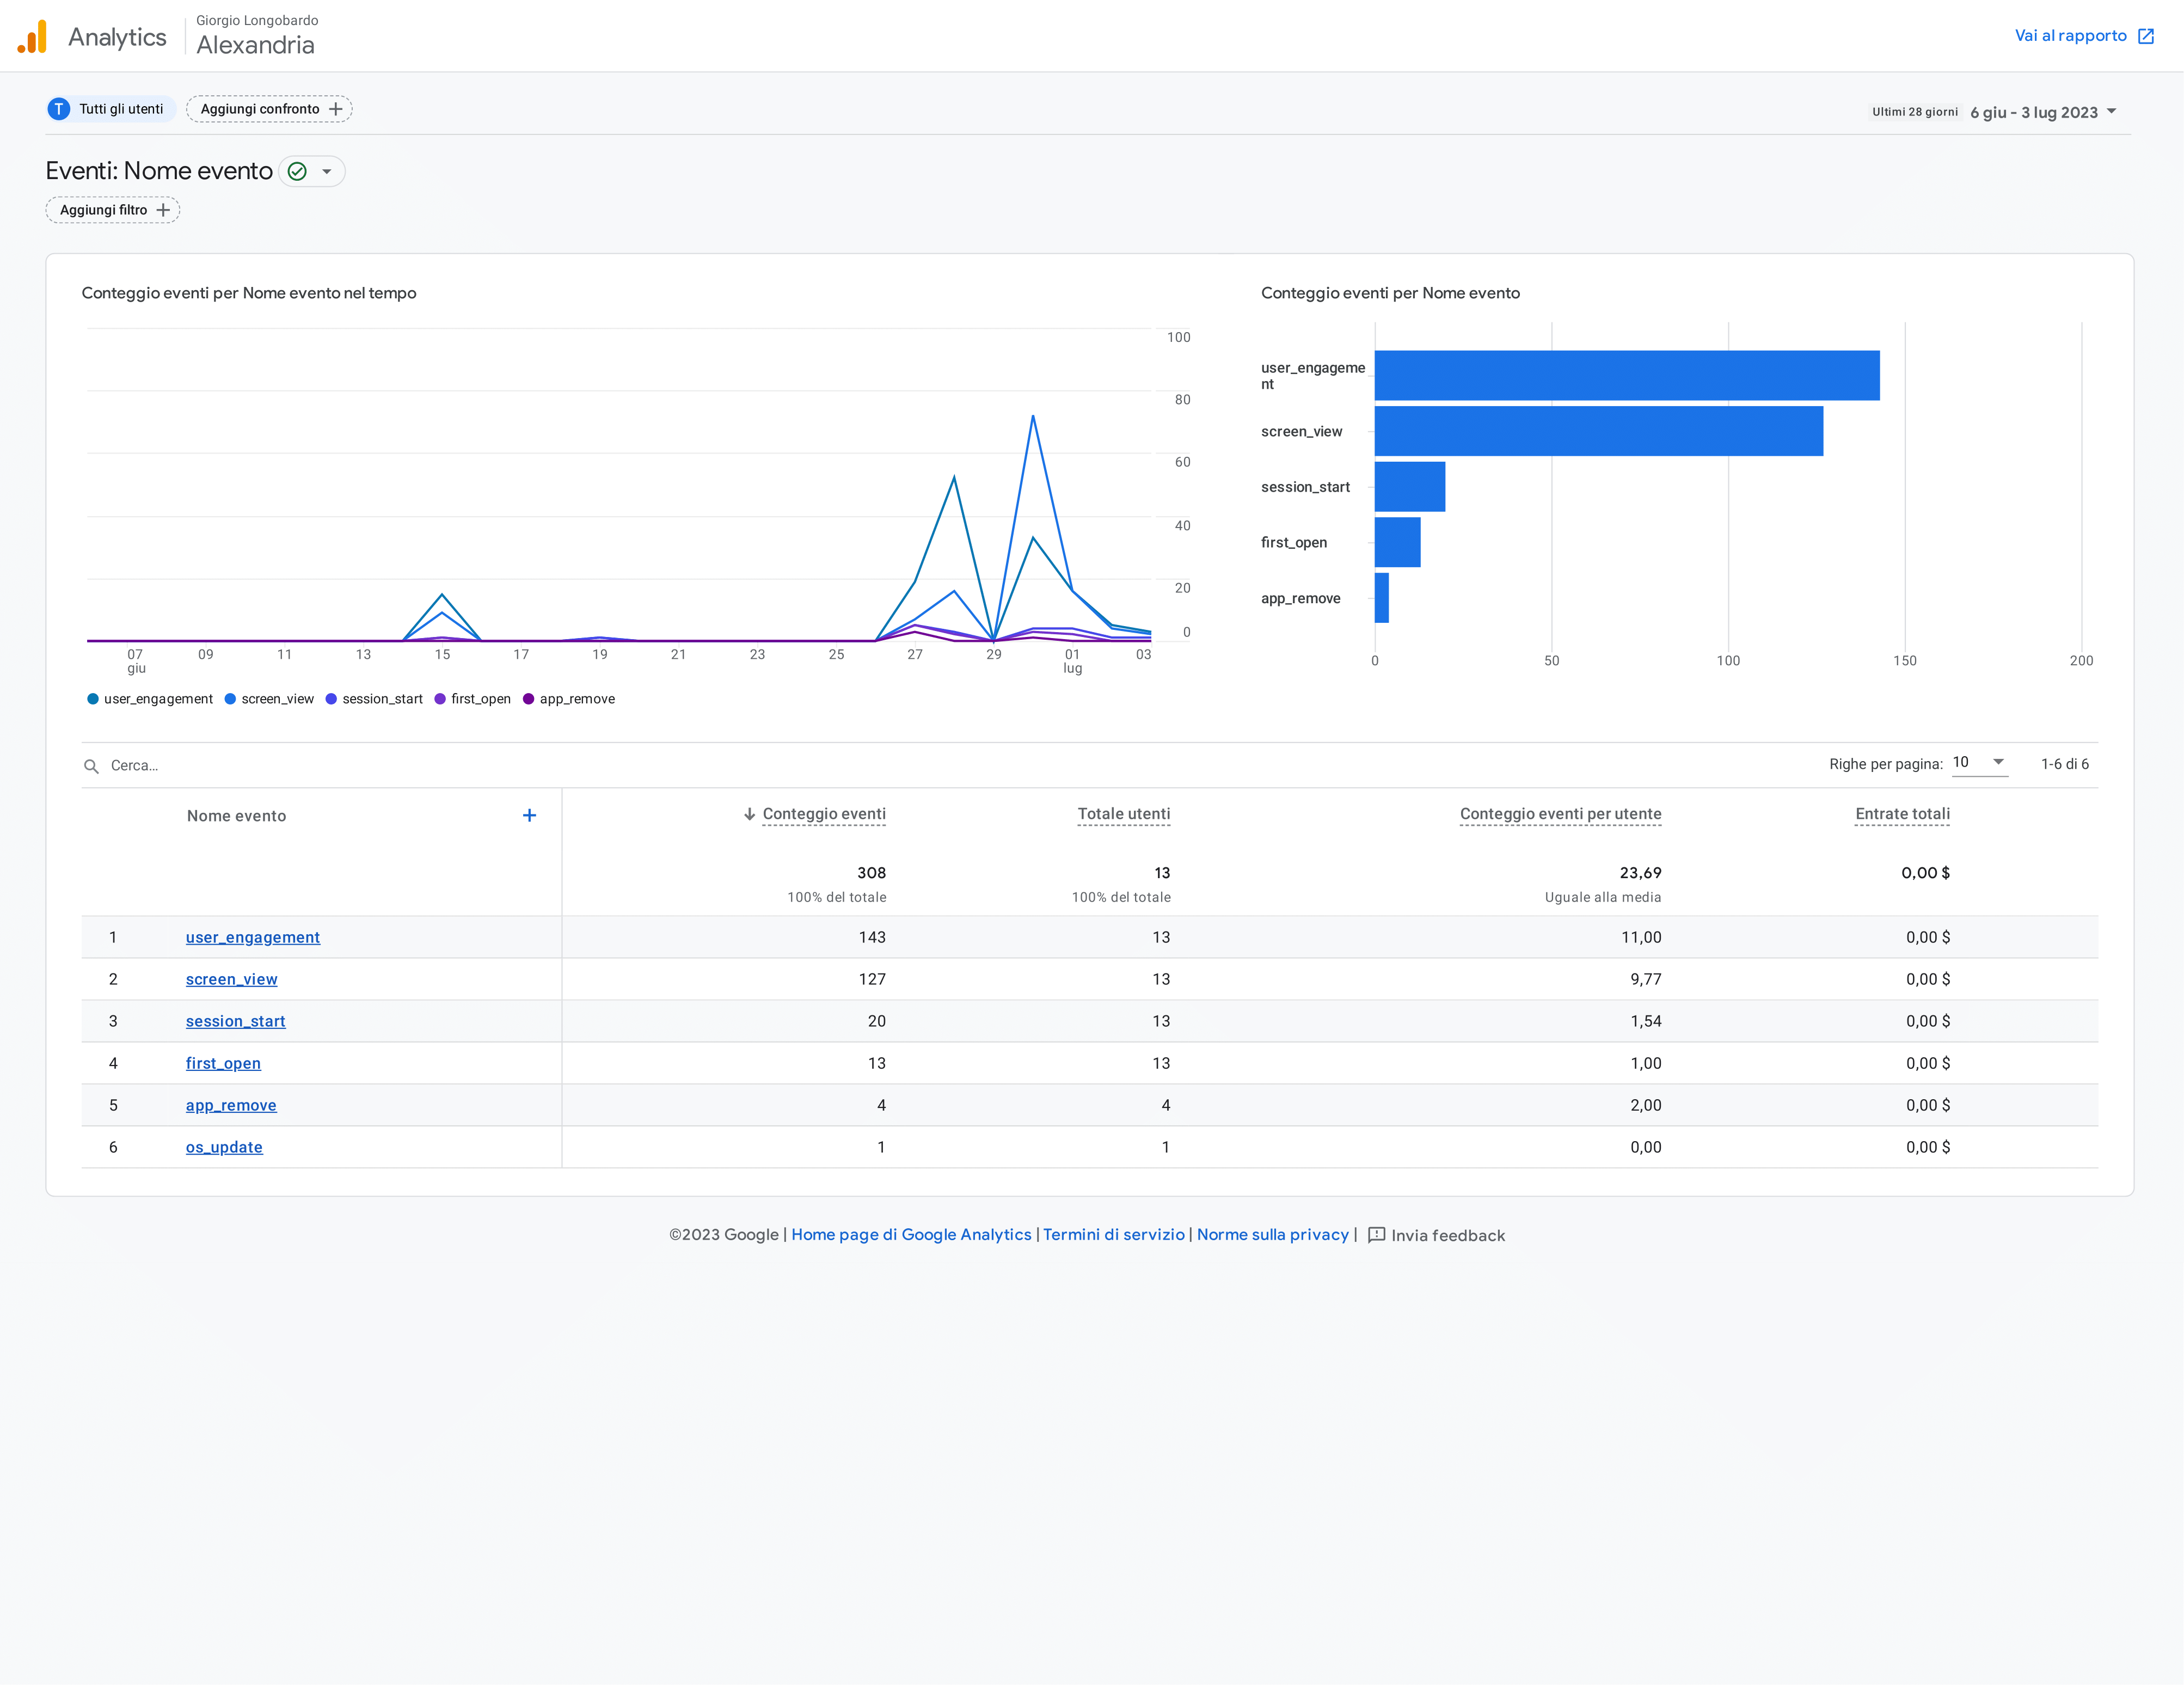
\includegraphics[width=0.99\textwidth]{Immagini/Alexandria/Report/eventi-1.png}
    \caption{Panoramica degli eventi}
\end{figure}

\begin{figure}[H]
    \centering
    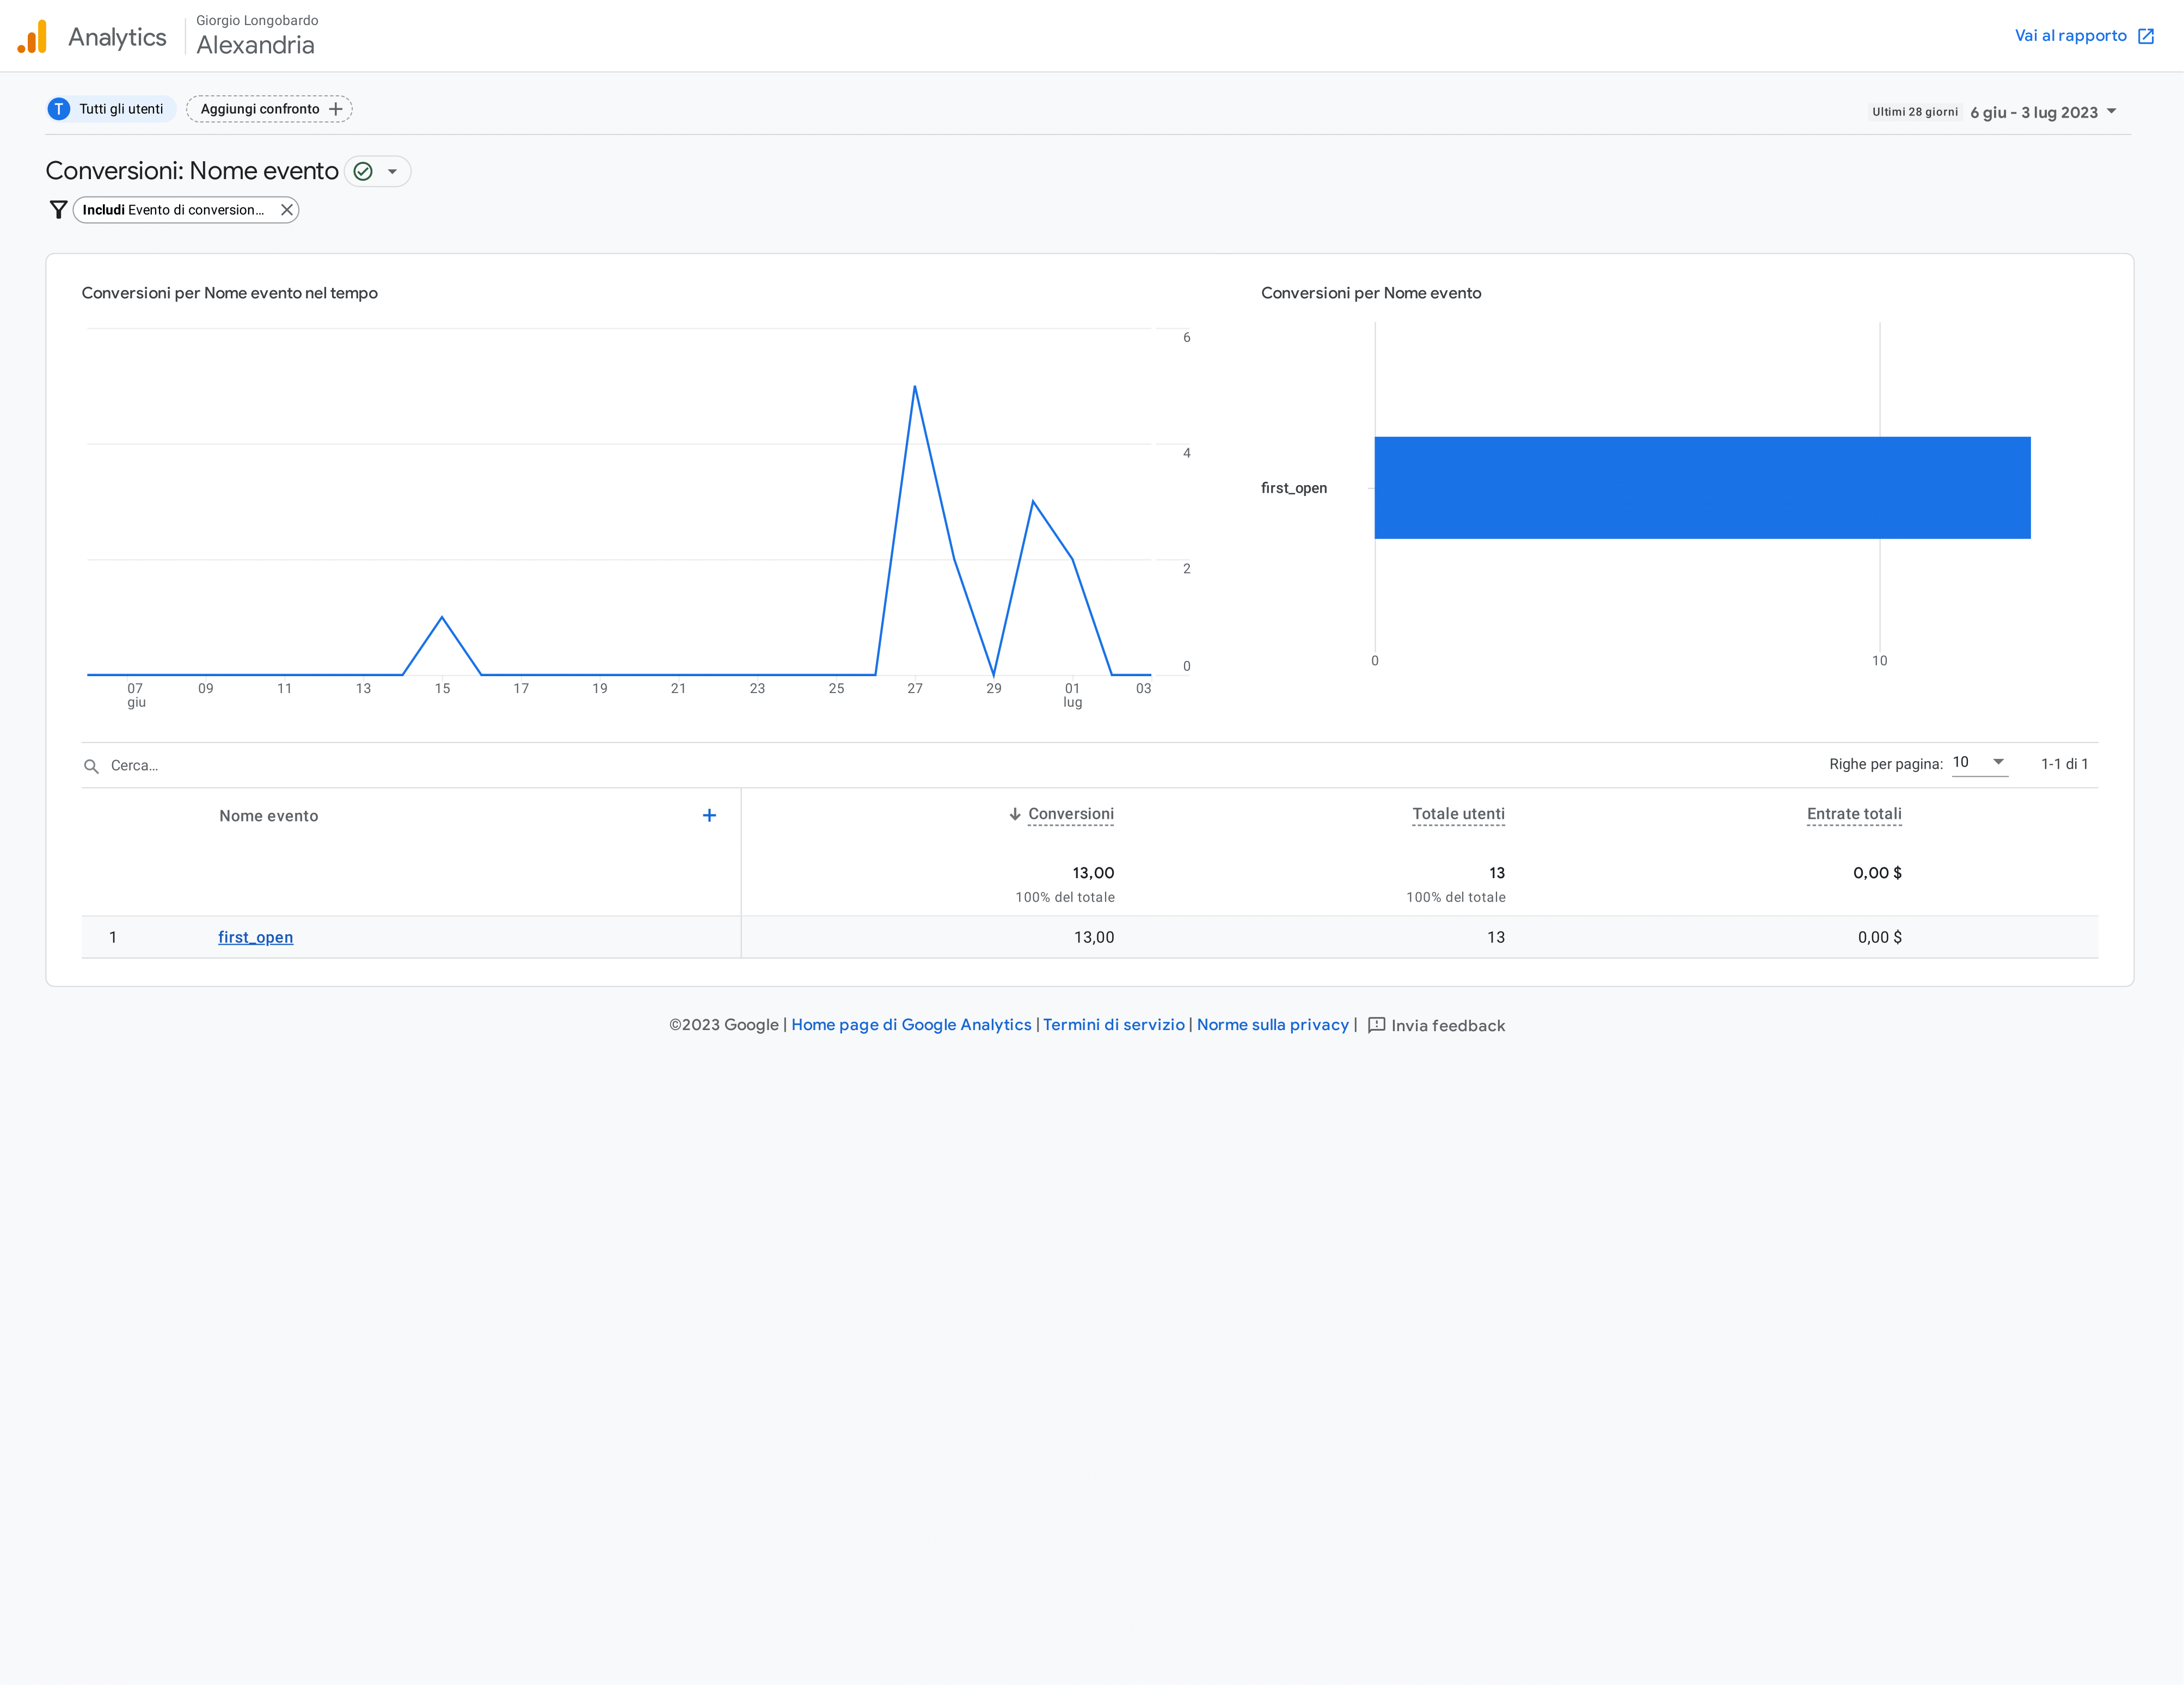
\includegraphics[width=0.99\textwidth]{Immagini/Alexandria/Report/conversioni-1.png}
    \caption{Panoramica delle conversioni}
\end{figure}

\begin{figure}[H]
    \centering
    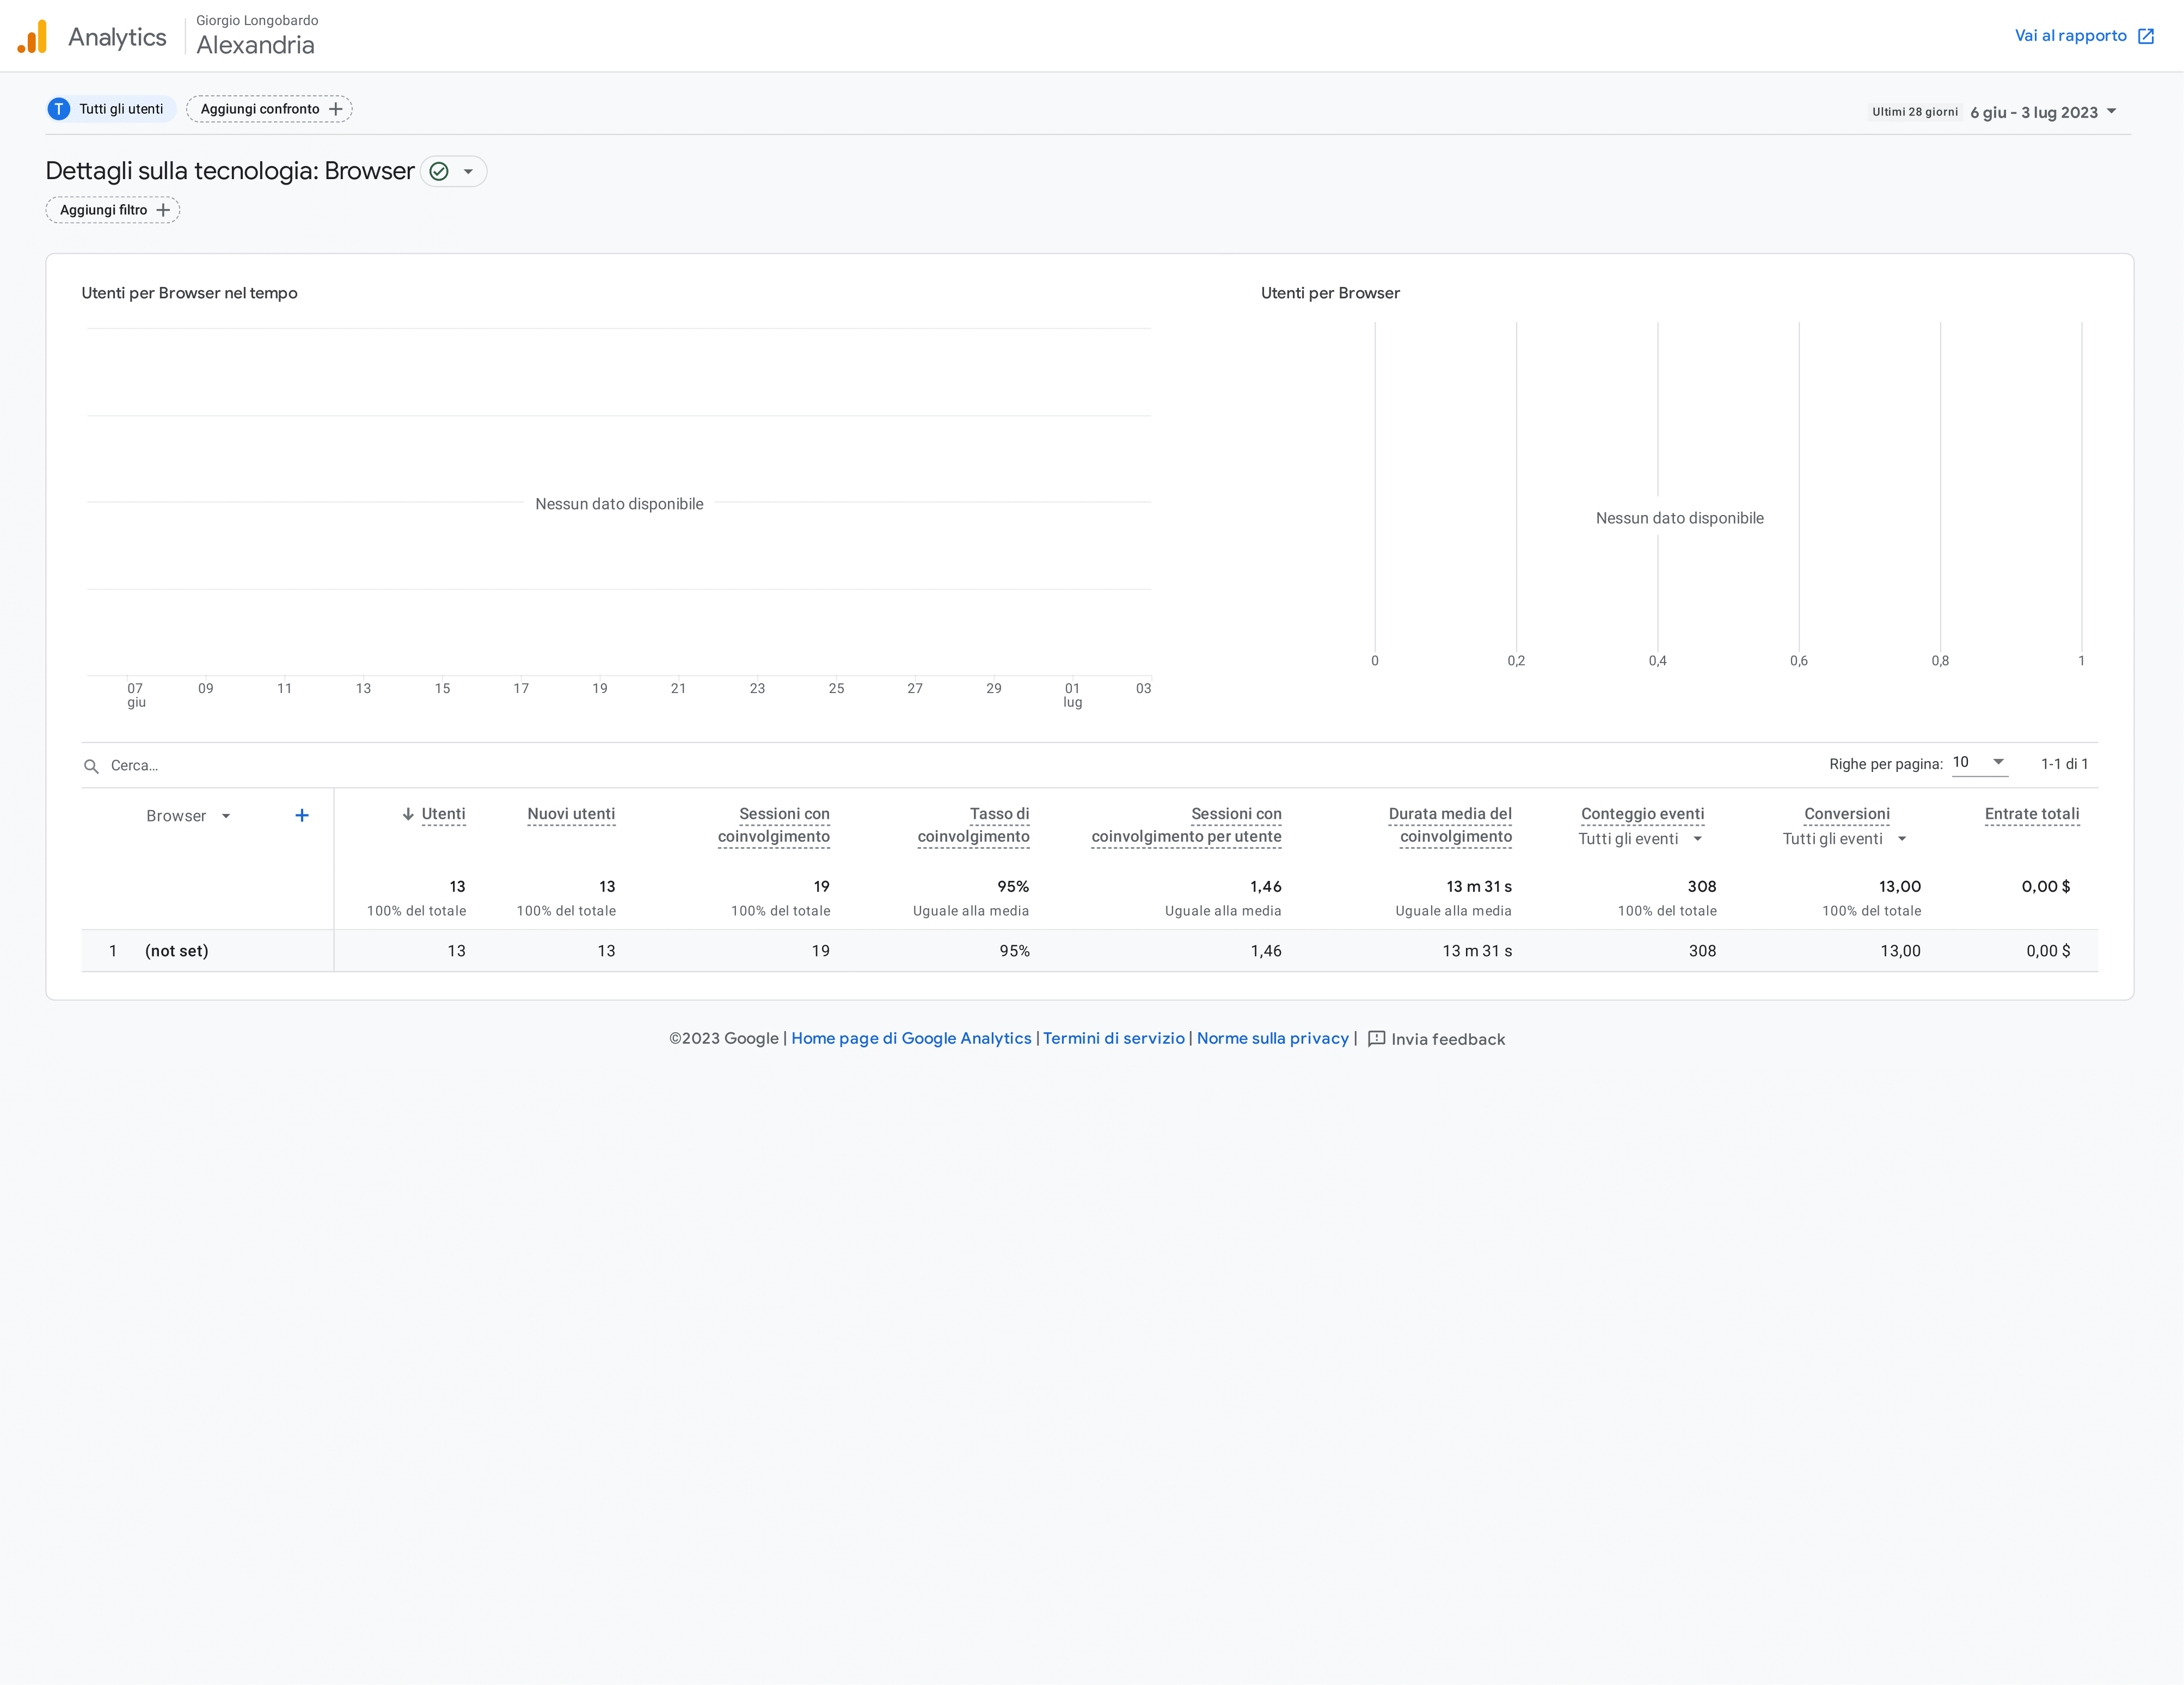
\includegraphics[width=0.99\textwidth]{Immagini/Alexandria/Report/dettagliTecnologia-1.png}
    \caption{Panoramica dettagli delle tecnologie}
\end{figure}

In particolare, abbiamo deciso principalmente di apportare due modifiche all'applicativo finale: la gradazione del colore principale dell'applicazione e migliorie alle schermate di controllo per aumentare \textit{l'affordance.} Abbiamo deciso di tenere traccia dei tasso di successo di pochi utenti per poi modificare eventualmente l'applicativo rendendolo più semplice. Ergo è stata compilata questa tabella:

\begin{table}[h]
\resizebox{\columnwidth}{!}{\begin{tabular}{|l|c|c|c|c|c|c|}
\hline
                      & \multicolumn{1}{l|}{Task 1: Ricerca Riferimento} & \multicolumn{1}{l|}{Task 2: Creazione Riferimento} & \multicolumn{1}{l|}{Task 3: Creazione Categoria} & \multicolumn{1}{l|}{Task 4: Modifica Riferimento} & \multicolumn{1}{l|}{Task 5: Visualizzazione di un Riferimento} & \multicolumn{1}{l|}{Task 6: Eliminazione Riferimento} \\ \hline
Utente 1              & S                                                & S                                                  & S                                                & P                                                 & S                                                              & S                                                     \\ \hline
Utente 2              & S                                                & S                                                  & P                                                & F                                                 & S                                                              & S                                                     \\ \hline
Utente 3              & S                                                & S                                                  & S                                                & S                                                 & S                                                              & S                                                     \\ \hline
Utente 4              & S                                                & S                                                  & S                                                & P                                                 & S                                                              & S                                                     \\ \hline
Utente 5              & S                                                & S                                                  & S                                                & P                                                 & S                                                              & P                                                     \\ \hline
Percentuale successo: & 100\%                                            & 100\%                                              & 90\%                                             & 45\%                                              & 100\%                                                          & 90\%                                                  \\ \hline
\end{tabular}}
\caption{Tasso di successo}
\end{table}
Dove S, F e P indicano rispettivamente Successo, Fallimento e Parziale (Successo). E' da precisare inoltre che la tabella non tiene conto del tempo impiegato per ogni utente a svolgere un determinato compito. Tutti gli utenti rivestono il ruolo di un normale utente, non godendo di particolari privilegi del sistema, ma solamente eventuale potere di creare categorie, riferimenti ed eliminare i propri oggetti realizzati.

Una volta analizzati i dati, abbiamo deciso di migliorare le schermate dei Task che generassero un basso tasso di successo. In questo caso, il compito \textit{Modifica Riferimento} genera un tasso di successo < 60\%, dove 60 è un tasso che consideriamo sufficiente per non modificare le schermate correlate. Dunque, la schermata per la modifica di un riferimento ha subito migliorie per evitare fraintendimenti o casi di insuccesso. 
